\chapter{Tarea 4}

\framedt{Tarea a realizar}{
   Visualiza el siguiente vídeo:
   \href{
      www.youtube.com/watch?v=8edHD2o0pao
   }{youtube.com/watch?v=8edHD2o0pao}
   
   Contesta a las siguientes preguntas:
   \begin{itemize}
   	\item Explica las medidas que propone el video para securizar un sistema de Smart Grid
	   \item Sugiere alguna medida adicional no recogida en el vídeo  
   \end{itemize}
}
\vspace{2em}

\section{Introducción}
La \textit{``low voltage smart grid''} es un soft target que es de importancia crítica para el suministro de \textit{Energía Sostenible} y las \textit{DSO's Billing Operations} (``Operador del Sistema de Distribución'').
\note{Ejemplos de tales operaciones incluyen la gestión de recursos energéticos distribuidos (DERs), recarga de vehículos eléctricos (EV), y sistemas de gestión energética del hogar (HEMS).}

\section{Medidas para Asegurar una Smart Grid}
El vídeo sugiere seis pasos clave que deben tomar todas las partes involucradas en el suministro para ser robustas frente a ciberataques:
\begin{enumerate}
   % \item \ul{``El \textbf{cumplimiento normativo} y la \textbf{protección} deben considerarse el \textit{mínimo}, no el nivel \textit{deseado} de seguridad''}\\
   \item \ul{``\textbf{Regulatory compliance} and \textbf{protection} should be considered the \textit{minimum}, not the \textit{desired} level of security''}\\
   Esto ayuda a pensar como un cibercriminal y anticipar sus acciones.
   % \item \ul{``No confíes en la \textbf{opcionalidad} en seguridad}\\
   \item \ul{``Don't trust \textbf{optionality} in security}\\
   Los cibercriminales buscan medidas de seguridad \textit{opcionales} para explotar. Si una medida de seguridad es opcional, es probable que sea ignorada por algunas partes, lo que puede conducir a vulnerabilidades, potencialmente permitiendo a los criminales infiltrarse y desactivar incluso las medidas de seguridad obligatorias.
   % \item \ul{``No asumas que tu seguridad es \textbf{única} y que esto te protege''}\\
   \item \ul{``Don't assume your security is \textbf{unique} and that this protects you''}\\
   Los cibercriminales siempre tienen varias herramientas a su disposición, y no dudarán en usarlas. Incluso si piensas que tus medidas de seguridad son únicas, aún pueden ser evadidas por un atacante determinado.\\
   Los DSO deberían realizar \textbf{Pruebas de Penetración} (PT) regularmente para evaluar la eficacia de sus medidas de seguridad, preferiblemente por probadores con experiencia en redes inteligentes de baja tensión.\footnote{low voltage smart grids}
   % \item \ul{``\textit{Invertir} en \textbf{detección y respuesta ante amenazas}''}\\
   \item \ul{``\textit{Invest} in \textbf{threat detection and response}''}\\
   Esto permitiría al equipo de seguridad centrarse en los ataques organizados, como ataques de Ransom o de Denial of Service (DoS), que son más propensos a tener éxito y causar daños significativos.\\
   Además, una detección robusta es síntoma de \textit{``saber lo que pasa''}, es decir, \textit{Ciberconciencia Situacional}, que es un elemento clave de cualquier estrategia de seguridad.
   % \item \ul{``Proporcionar un \textbf{disuasivo} efectivo''}\\
   \item \ul{``Provide an effective \textbf{deterrent}''}\\
   Explotar las capacidades de detección y respuesta para disuadir a los cibercriminales y construir un conjunto de evidencias contra ellos.\\
   Esto se puede lograr implementando medidas como \textbf{Honeypots} y \textbf{Honeynets}, que están diseñadas para atraer y atrapar a los cibercriminales, permitiendo a los equipos de seguridad recopilar información sobre sus tácticas y técnicas.
   % \item \ul{``\textbf{Integra} tu red inteligente de baja tensión con tu \textbf{seguridad corporativa}''}\\
   \item \ul{``\textbf{Integrate} your low voltage smart grid with your \textbf{corporate security}''}\\
   Esto permitiría al equipo de seguridad tener una visión holística de la postura de seguridad de la organización, facilitando la identificación de ataques multipunto y la coordinación de la respuesta a los mismos.
\end{enumerate}

En última instancia, el vídeo nos recuerda que todos somos víctimas potenciales de ciberataques, sin importar lo débiles o fuertes que sean nuestras medidas de seguridad.\\
Al fin y al cabo, el punto clave es tener personas, organizaciones y tecnologías en tu organización que puedan pensar como un cibercriminal.

\section{Medidas Adicionales}

Además de las medidas propuestas en el vídeo, existen otras estrategias complementarias que podrían fortalecer significativamente la seguridad de una Smart Grid:

\begin{enumerate}
   \begin{paracol}{2}
      \colfill
      \item \textbf{Implementación de blockchain}: Esta tecnología puede proporcionar una capa adicional de seguridad para la autenticación de transacciones energéticas y la protección de datos de medición, creando un registro inmutable de todas las operaciones.\\
      Esto es un poco más difícil de exploitar por un atacante, y podría ayudar a garantizar la integridad de los datos al menos para algunas operaciones, contrarrestando el riesgo de manipulación de datos..
      \colfill
      
      \switchcolumn

      \begin{figure}[htbp]
         \centering
         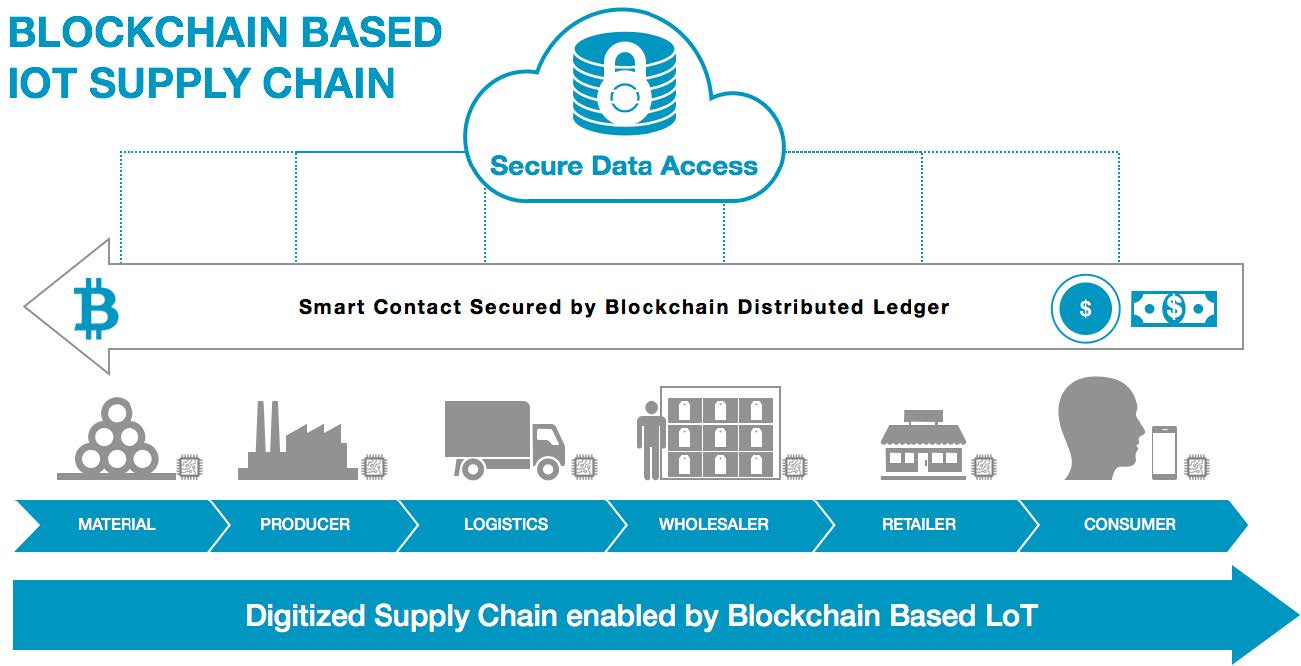
\includegraphics[width=0.95\columnwidth]{images/blockchain.jpg}
         \caption{Ejemplo de blockchain tracked supply chain}
         \label{fig:blockchain}
      \end{figure}
   \end{paracol}
   
   \item \textbf{Segmentación de red avanzada}: Dividir la red en zonas aisladas para contener posibles brechas de seguridad, limitando el movimiento lateral de los atacantes mediante técnicas de microsegmentación.\\
   Se supone que esto está sobreentendido en el vídeo, pero aun así es importante mencionarlo.
   
   \begin{paracol}{2}
      
      \colfill
      \item \textbf{Simulación del estado esperado de la red}:
      Simular el estado esperado de la red para detectar desviaciones que puedan indicar un ataque en curso. Esto puede incluir la monitorización de patrones de tráfico y el uso de inteligencia artificial para identificar anomalías.\\
      Algo similar a lo que se hace para sistemas idraulicos con \texttt{epanetCPA}, pero aplicado a la red eléctrica.

      Esto se puede juntar a medidas de analisis de riesgo dinámico, que permiten actualizar continuamente la evaluación de riesgos basándose en datos en tiempo real sobre amenazas, vulnerabilidades y cambios en la infraestructura.
      \colfill

      \switchcolumn

      \begin{figure}[htbp]
         \centering
         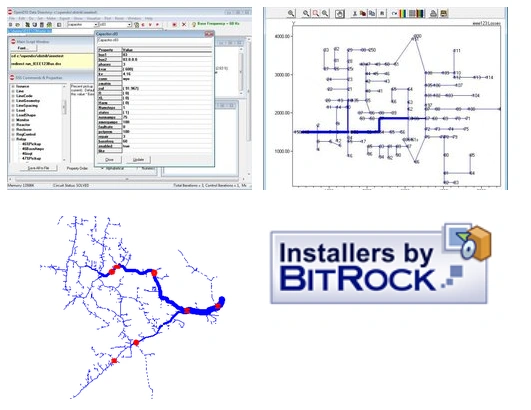
\includegraphics[width=0.95\columnwidth]{images/opendss.png}
         \caption{OpenDSS, un simulador de sistemas eléctricos de distribución.}
         \label{fig:opendss}
      \end{figure}
   \end{paracol}




   \item \textbf{Asegurar autenticación y autorización robustas para activos críticos}: Implementar autenticación multifactor (MFA) y controles de acceso basados en roles para garantizar que solo los usuarios autorizados puedan acceder a sistemas críticos.
   
   \newpage
   \begin{paracol}{2}
      \colfill
      \item \textbf{Modelado de Attack Graphs específicos para Smart Grids}: Desarrollar representaciones gráficas que muestren cómo los atacantes podrían explotar vulnerabilidades interconectadas en sistemas SCADA, medidores inteligentes y redes de comunicación, facilitando la identificación de puntos críticos de fallo.
      \colfill
      
      \switchcolumn

      \begin{figure}[htbp]
         \centering
         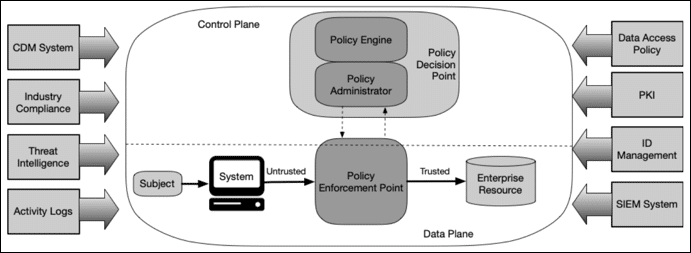
\includegraphics[width=0.95\columnwidth]{images/zta.png}
         \caption{Ejemplo de Zero Trust Architecture (ZTA), un paradigma de seguridad que asume que las amenazas pueden estar tanto dentro como fuera de la red, y por lo tanto requiere autenticación y autorización estrictas para cada acceso a recursos.}
         \label{fig:zta}
      \end{figure}
   \end{paracol}
   

   % \item \textbf{Análisis de comportamiento de usuarios y entidades (UEBA)}: Implementar sistemas que establezcan líneas base de comportamiento normal para detectar anomalías que podrían indicar compromisos de seguridad.
   
   % \item \textbf{Redundancia de sistemas críticos}: Establecer sistemas redundantes geográficamente distribuidos para mantener la operatividad frente a ataques dirigidos a componentes específicos.
   
   % \item \textbf{Ejercicios de simulación de crisis}: Realizar simulacros regulares de ciberataques para evaluar la respuesta de la organización y mejorar los protocolos de actuación.
   
   % \item \textbf{Colaboración público-privada}: Establecer canales de comunicación con organismos gubernamentales y otras empresas del sector para compartir información sobre amenazas emergentes y coordinar respuestas.

   % \item \textbf{Cifrado de extremo a extremo para comunicaciones críticas}: Implementar protocolos de cifrado robusto para todas las comunicaciones entre dispositivos IoT, contadores inteligentes y sistemas de control, protegiendo los datos en tránsito contra interceptación y manipulación.
   
   % \item \textbf{Gestión de identidades de dispositivos IoT}: Establecer un sistema centralizado de gestión de identidades para todos los dispositivos conectados, con certificados digitales únicos y rotación periódica de credenciales para prevenir la suplantación de dispositivos.
   
   % \item \textbf{Monitorización del tráfico de red en tiempo real}: Implementar sistemas de análisis de tráfico que puedan detectar patrones anómalos, comunicaciones no autorizadas o intentos de exfiltración de datos mediante técnicas de \textit{Deep Packet Inspection} (DPI).
   


   \item \textbf{Actualizaciones de firmware automatizadas y seguras}: Desarrollar mecanismos de actualización automática con verificación criptográfica para mantener todos los dispositivos de la red actualizados contra vulnerabilidades conocidas, incluyendo sistemas de rollback en caso de fallos.\\
   Esto suele ser especialmente complicado en dispositivos IoT y Legacy, pero es crucial para mantener la seguridad a largo plazo.
   
   % \item \textbf{Análisis forense digital preparatorio}: Establecer capacidades de análisis forense digital proactivo, incluyendo logging detallado y herramientas de análisis que permitan una investigación rápida y efectiva en caso de incidente.
   
   % \item \textbf{Controles de integridad de firmware}: Implementar verificaciones periódicas de integridad del firmware en dispositivos críticos para detectar modificaciones maliciosas o compromisos a nivel de hardware.

   \item \textbf{UEBA} (\textit{User and Entity Behavior Analytics}) para Smart Grids: Implementar sistemas que establezcan líneas base de comportamiento normal para detectar anomalías que podrían indicar compromisos de seguridad, especialmente en dispositivos IoT y sistemas SCADA.\\
   Dado que las redes inteligentes tienen probablemente un conjunto estándar de operaciones, ésta podría ser una buena forma de detectar anomalías en el sistema y, por tanto, posibles ataques.
   
   \item \textbf{Planificación de continuidad de negocio específica para ciberataques}: Desarrollar planes específicos de recuperación ante desastres cibernéticos que incluyan procedimientos de operación manual temporal y criterios claros para la reconexión de sistemas tras un ataque.
   
   \begin{paracol}{2}
      \colfill   
      \item \textbf{Aislamiento físico de sistemas críticos}: Mantener sistemas de control críticos en redes físicamente separadas (\textit{air-gapped}) cuando sea posible, especialmente para operaciones de protección y control de emergencia.
      \colfill   
      \switchcolumn
      \begin{figure}[htbp]
         \centering
         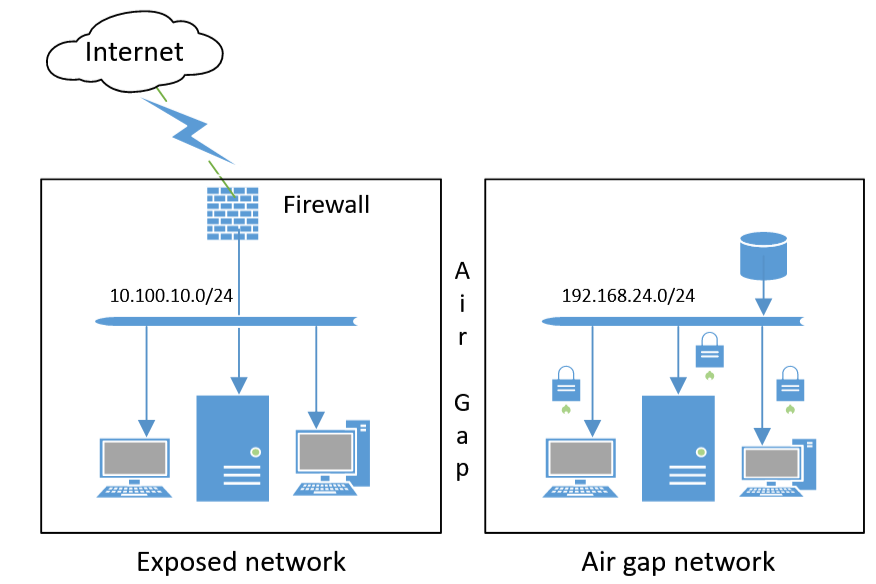
\includegraphics[width=0.95\columnwidth]{images/airgap.png}
         \caption{Air Gapped network topology example.}
         \label{fig:airgap}
      \end{figure}
   \end{paracol}
   \item \textbf{Implementación de un Common Operational Picture (COP) para Smart Grids}: Establecer una vista única y compartida de la situación operativa que integre datos de la red eléctrica, sistemas de control y sensores de seguridad, permitiendo que todos los operadores tengan la misma conciencia situacional en tiempo real.\\
   Esto se relaciona con la integración de la red inteligente con la seguridad corporativa mencionada en el vídeo, pero se centra más en la creación de una imagen operativa común que facilite la toma de decisiones informadas y coordinadas.
   
   % \item \textbf{Análisis de riesgo dinámico}: Implementar sistemas que actualicen continuamente la evaluación de riesgos basándose en datos en tiempo real sobre amenazas, vulnerabilidades y cambios en la infraestructura, superando las limitaciones de los análisis estáticos tradicionales.
   
   % \item \textbf{Integración de inteligencia de amenazas externa}: Incorporar feeds de ciberinteligencia (OSINT, HUMINT, SIGINT, TECHINT) utilizando estándares como STIX/TAXII para mantenerse actualizado sobre amenazas emergentes específicas a infraestructuras críticas energéticas.
   
   
   % \item \textbf{Georreferenciación de activos críticos}: Vincular todos los componentes digitales de la Smart Grid con su ubicación física precisa, permitiendo correlacionar incidentes cibernéticos con eventos físicos locales y mejorar la respuesta coordinada entre equipos técnicos y de seguridad.
   
   % \item \textbf{Implementación de niveles de CS estratégico, operativo y táctico}: Estructurar la información de seguridad en tres niveles jerárquicos - desde detalles técnicos específicos para respuesta inmediata hasta análisis estratégicos para planificación a largo plazo - asegurando que cada nivel decisional reciba información apropiada.
   
   % \item \textbf{Sistemas de gestión de sobrecarga informativa}: Implementar filtros inteligentes y técnicas de priorización para evitar que los operadores se vean abrumados por alertas, utilizando Mission Awareness para determinar qué información es crítica según el contexto operativo específico.

\end{enumerate}

Estas medidas adicionales, junto con las mencionadas en el vídeo, conformarían una estrategia de defensa en profundidad más robusta, aumentando significativamente la resiliencia de la Smart Grid frente a ciberataques cada vez más sofisticados.